\documentclass[a4paper,UKenglish]{lipics-v2016}
%This is a template for producing LIPIcs articles. 
%See lipics-manual.pdf for further information.
%for A4 paper format use option "a4paper", for US-letter use option "letterpaper"
%for british hyphenation rules use option "UKenglish", for american hyphenation rules use option "USenglish"
% for section-numbered lemmas etc., use "numberwithinsect"
 
\usepackage{microtype}%if unwanted, comment out or use option "draft"

%\graphicspath{{./graphics/}}%helpful if your graphic files are in another directory

\bibliographystyle{plainurl}% the recommended bibstyle

% Author macros::begin %%%%%%%%%%%%%%%%%%%%%%%%%%%%%%%%%%%%%%%%%%%%%%%%
\title{Interactive Geometric Algorithm Visualization in a Browser\footnote{This work was partially supported by the National Science Foundation under grant CCF-1525978.}}
\titlerunning{Interactive Geometric Algorithm Visualization} %optional, in case that the title is too long; the running title should fit into the top page column

%% Please provide for each author the \author and \affil macro, even when authors have the same affiliation, i.e. for each author there needs to be the  \author and \affil macros
\author[1]{Lynn Asselin}
\author[2]{Kirk P. Gardner}
\author[3]{Donald R.~Sheehy}
\affil[1]{University of Connecticut\\
  \texttt{lynn.asselin@uconn.edu}}
\affil[2]{University of Connecticut\\
  \texttt{kirk.gardner@uconn.edu}}
\affil[3]{University of Connecticut\\
  \texttt{don.r.sheehy@gmail.com}}

\authorrunning{L.\,Asselin, K.\,P.\,Gardner, and D.\,R.\,Sheehy} %mandatory. First: Use abbreviated first/middle names. Second (only in severe cases): Use first author plus 'et. al.'

\Copyright{Lynn Asselin, Kirk P. Gardner, and Donald R.~Sheehy}%mandatory, please use full first names. LIPIcs license is "CC-BY";  http://creativecommons.org/licenses/by/3.0/

\subjclass{F.2.2 Nonnumerical Algorithms and Problems---Geometrical problems and computations.}
% \subjclass{F.2.2 Nonnumerical Algorithms and Problems}% mandatory: Please choose ACM 1998 classifications from http://www.acm.org/about/class/ccs98-html . E.g., cite as "F.1.1 Models of Computation".
\keywords{Computational Geometry, Processing, JavaScript, Visualisation, Incremental Algorithms}% mandatory: Please provide 1-5 keywords

\EventEditors{S\'andor Fekete and Anna Lubiw}
\EventNoEds{2}
\EventLongTitle{32nd International Symposium on Computational Geometry
(SoCG 2016)}
\EventShortTitle{SoCG 2016}
\EventAcronym{SoCG}
\EventYear{2016}
\EventDate{June 14-18, 2016}
\EventLocation{Boston, USA}
\EventLogo{}
\SeriesVolume{51}
\ArticleNo{64}    %Proceedings number goes here!

% Author macros::end %%%%%%%%%%%%%%%%%%%%%%%%%%%%%%%%%%%%%%%%%%%%%%%%%

% %Editor-only macros:: begin (do not touch as author)%%%%%%%%%%%%%%%%%%%%%%%%%%%%%%%%%%
% \serieslogo{}%please provide filename (without suffix)
% \volumeinfo%(easychair interface)
%   {Billy Editor and Bill Editors}% editors
%   {2}% number of editors: 1, 2, ....
%   {Conference title on which this volume is based on}% event
%   {1}% volume
%   {1}% issue
%   {1}% starting page number
% \EventShortName{}
% \DOI{10.4230/LIPIcs.xxx.yyy.p}% to be completed by the volume editor
% % Editor-only macros::end %%%%%%%%%%%%%%%%%%%%%%%%%%%%%%%%%%%%%%%%%%%%%%%

\begin{document}

\maketitle

\begin{abstract}
  We present an online, interactive tool for writing and presenting interactive geometry demos suitable for classroom demonstrations.
  Code for the demonstrations is written in JavaScript using \texttt{p5.js}, a JavaScript library based on Processing.
\end{abstract}

\section{Motivation} % (fold)
\label{sec:motivation}

  At CG Week 2013 in Rio de Janeiro, Suresh Venkatasubramanian presented at the Workshop on Geometric Computing Challenges with a strong plea for more and better tools for producing interactive pedagogical geometry demos.  
  In his abstract\footnote{\url{http://zeus.mat.puc-rio.br/~socg2013/index.php/workshops/geometric-computing-challenges\#abstract-suresh}} he describes the situation quite clearly:
  \begin{quote}    
    The early days of the Web were a goldmine for geometric algorithm demos. The visual and interactive nature of geometric algorithms, coupled with the proliferation of lightweight Java applets, made the HTML canvas a fantastic portable framework for teaching and demonstrations.

    Fast forward to 2013. We have a blizzard of Javascript frameworks, sophisticated HTML5 based in-browser animations, and a host of new platforms on which to demo algorithms. We also have a mature geometric computing platform in the form of CGAL. But we no longer have geometric demos that work well (or at all in many cases).
  \end{quote}

  Here in 2016, the situation is not much different.
  In this paper, we describe a tool that fills this gap.
  It is informed by experience collected from teaching an introductory course on Computational Geometry at the University of Connecticut in which students produced such demos as course projects.
  In most cases, the challenges of \textbf{dealing with interaction and visualization dominated the geometric ideas}.

  \clearpage
  Our interactive geometric algorithm visualizer is designed with the following goals.
  \begin{enumerate}
    \item It should be possible to visualize a geometric algorithm without writing any explicit visualization code.  
    \item It should be possible to produce an interactive (incremental) demonstration without writing any explicit code to deal with interaction.  
  \end{enumerate}
  
  Satisfying these two goals implies that all of the visualization and interaction code is abstracted away from the user, who is presented with a simple editor and a canvas.
  When more complex interaction or visualization is desired, access to these elements is available.
  
  The project is in active development, and the source code is available at \url{https://github.com/compugeom/compugeom.github.io}.  
  A live, interactive sandbox is available at \url{http://compugeom.github.io}.
  
  % We also expose enough of the visualiation and interaction elements to allow for more complex demos where the defaults do not suffice.
  
  % Lost applets
  % desire to connect code with visualization without writing a lot of viz. code
  % suitable for in-class demos
  % Event-driven interaction

% section motivation (end)

\section{Geometric Primitives} % (fold)
\label{sec:geometric_primitives} 

  Drawable classes take the form of primitives as well as data structures, and can be instantiated as geometric objects complete with visualization specifications, as well as any support functions needed to concisely represent the underlying mathematics.
  These provide a foundation for other data structures and algorithms to be built upon, as well as a natural way to abstract away visualization.
  The main objects currently provided are:
  \begin{itemize}
    \item Vertices, Edges and Faces - Objects which encapsulate \texttt{p5.js} primitives such as \emph{point} and \emph{line} that can be instantiated, visualized, and modified.
    \item Point sets - In particular, we allow for dynamic point sets which are generated by user input.
    \item Polygons - Our polygon implementation provides a cyclic Edge list data structure, and allows for easy indexing into the vertices, automatically wrapping indices around using modular arithmetic.
    \item Planar Straight Line Graphs - A simple half-edge data structure is used to store and traverse the Edges of an embedded planar graph.
  \end{itemize}
  As our objective is to construct a means for computational geometers, students, and developers to visualize algorithms in a way that mirrors the elegance of the underlying mathematics, we adopt a hierarchical paradigm in order to minimize redundancy within the framework. 
  These objects therefore make extensive, but not unnecessary use of lower dimensional primitives and data structures, with visualizations and functionality building naturally off of their component parts.
  In addition to the classes listed above, we provide standard linear predicates such as triangle orientation tests (i.e.\ CCW tests).

% section geometric_primitives (end)
\section{Technical Details} % (fold)
\label{sec:technical_details}

  The main library used is \texttt{p5.js}~\cite{p5js}, a JavaScript implementation of the Processing software sketchbook.
  We also use the Ace code editor~\cite{ace} to provide interactive visualizations in the web-page.
  
  % Our goal in this project is not only to build a web-based pedagogical tool, but also to provide a comprehensive and intuitive computational geometry library that allows students, educators and developers to quickly and easily implement well known geometric procedures.
  There is often a tradeoff between power and ease of use.
  In order to give a good balance between the two, we attempted to focus on our target users, computational geometry students and educators.
  Thus, the technical decisions are motivated by pedagogical concerns.
  
  The \texttt{p5.js}\footnote{\url{https://p5js.org/}} library provides a pure JavaScript implementation of the Processing software sketchbook: an API for rendering graphics such as shapes, lines and ellipses in 2D and 3D.
  These objects are rendered by placing them in an event loop, however there are no geometric objects provided by the \texttt{p5.js} library.
  To implement geometric algorithms in \texttt{p5.js/Processing} the provided visualization primitives are wrapped by classes that encapsulate geometric primitives.
  These primitives are then packaged alongside linear predicates and geometric data structures to provide data abstraction and visualization.

  The first step in constructing such a framework is, therefore, to handle the instantiation and visualization of drawable objects.
  This is accomplished by wrapping the event loop in a data structure that maintains the order of execution and animation of our algorithm visualizer.
  Thus the \texttt{CG\_Environment} class serves to abstract away as much of the embedded event loop as possible without restricting the user's access to the \texttt{p5.js} library.
  We have also created geometric primitives as objects, each containing relevant (and natural) properties and functions, as well as the ability to draw themselves when instantiated by a \texttt{CG\_Environment} object.
  This is achieved by keeping matrix of objects \texttt{CG\_Environment.things} sorted by dimension that are to be drawn in the event loop.
  Objects can also be used strictly as data structures without visualization by instantiating them directly from the library, as in Figure~\ref{fig:demo}
  
% section technical_details (end)

\section{Example: Incremental Convex Hull} % (fold)
\label{sec:example_incremental_convex_hull}
  
  As a proof of concept, we give an example of a incremental algorithm for computing the convex hull of a set of points.
  Usually, the term \emph{incremental algorithm} means that the input is processed one element at a time.
  The primary invariant maintained after processing each element is that the state of the algorithm is a correct output if the current element were the last one.
  That is, the correctness condition stands in as a loop invariant.  
  An alternative view is that the input arrives online and as each new input arrives, we update the output.
  This is the more interactive version and it's the perspective we take.

  The \texttt{CG\_DynamicPointSet} class defines a point set for which new points are generated with a mouse click on the canvas.
  Upon user input the update function is called, passing the new point as a parameter.
  Thus, to write a program, one need only instantiate a new \texttt{DynamicPointSet}, a new \texttt{Polygon} (for the output), and write the update function.
  Some example code is given below.

\begin{verbatim}
  // this algorithm dynamically computes the convex hull of a point set.  
  demo.P = demo.DynamicPointSet();
  var H = demo.Polygon();
  // dynamically compute the convex hull of the point set
  demo.P.updateFunction = function(q) {
      if (H.VertexList.length < 2) {
        H.newVertex(q);
        return;
      }
      var left = -1, right = -1;
      for (var i = 0; i < H.VertexList.length; i++) {
        if (H.orient(i, i+1, q) && H.orient(i, i-1, q)){ right = i; }
        if (H.orient(i+1, i, q) && H.orient(i-1, i, q)){ left = i; }
      }
      // if q is outside the hull remove vertices and insert q
      if (left != -1 && right != -1) { H.replace(q, left, right); }
  };
\end{verbatim}

\begin{figure}[htbp]
  \centering 
  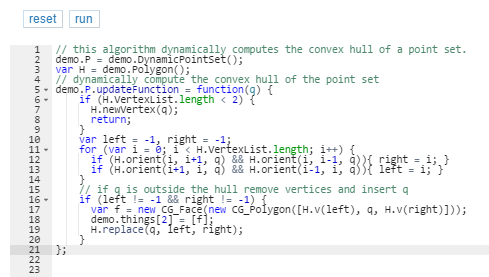
\includegraphics[scale=0.84]{figures/demo0.png}
  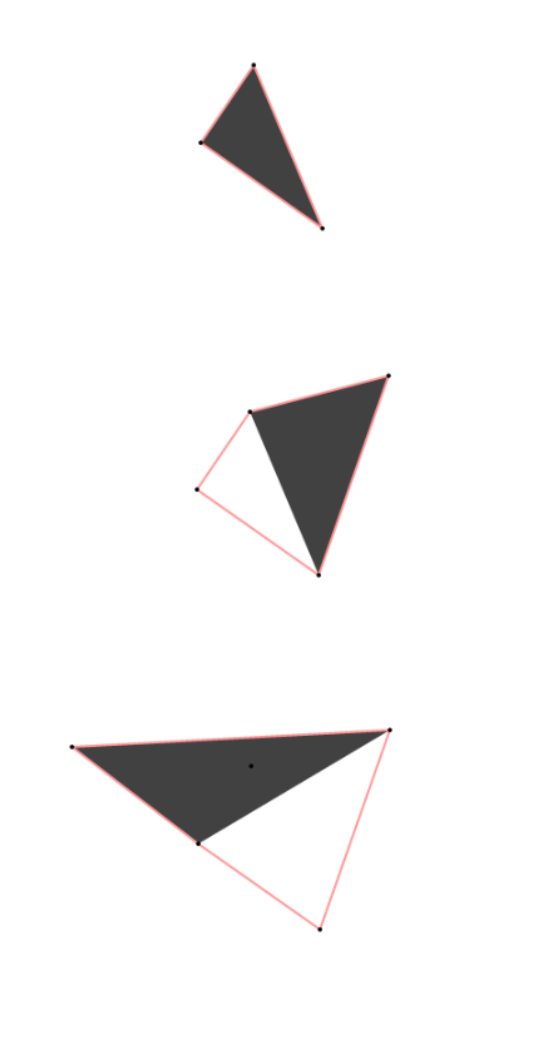
\includegraphics[scale=0.195]{figures/figs.png}
  % 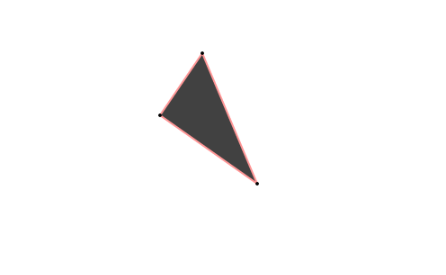
\includegraphics[scale=0.2]{figures/demo1.png}
  % 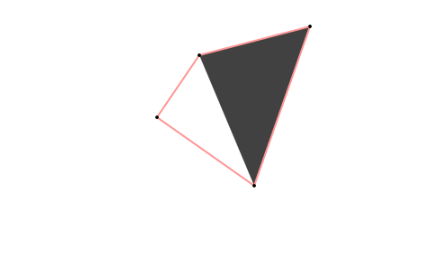
\includegraphics[scale=0.2]{figures/demo2.png}
  % 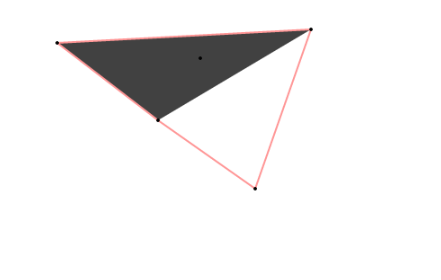
\includegraphics[scale=0.2]{figures/demo3.png}
  % 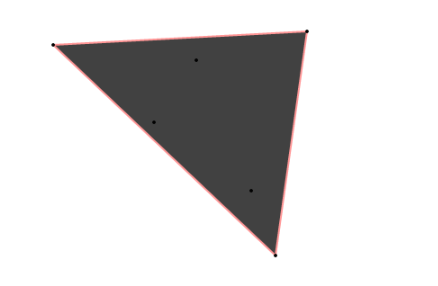
\includegraphics[scale=0.28]{figures/demo4.png}
  \caption{A screen capture from the live webpage (left) and several steps (right) of an augmented convex hull algorithm that visualizes the edited region of the polygon.
  It first constructs a face from \texttt{q} and the left and right-most remaining points, \texttt{var f = new CG\_Face(new CG\_Polygon([H.v(left), q, H.v(right)]))}, and sets it as the only 2D object that is to be drawn, \texttt{demo.things[2] = [f]}.}
  \label{fig:demo}
\end{figure}

  The demo object is an instance of the \texttt{CG\_Environment} class, and is used here to instantiate a \texttt{DynamicPointSet} to handle user input and a \texttt{Polygon}, the convex hull.
  The rest of the code is intended to be representative of the algorithm specification by making use of predicates and functions that are natural to the data types in question.

  Figure~\ref{fig:demo} illustrates a simple augmentation of the convex hull algorithm that makes use of the \texttt{CG\_Face} class, taken directly from the web-page.
  In contrast to the factory function provided by the \texttt{CG\_Environment} class, here we directly access the matrix, \texttt{CG\_Environment.things}, of drawn objects in order to ensure we only have one 2D object: the face that represents the most recent change in the hull.
  This is how the user can have more direct access to the underlying drawing, when it is desired.


% section example_incremental_convex_hull (end)

% \section{The Visualization Philosophy} % (fold)
% \label{sec:the_visualization_philosophy}
%
%   A key to achieving the design goal of having a minimum amount of visualization specific code cluttering the
%
%   Global Scope for viz elements
%   If it exists, it gets drawn by default

% section the_visualization_philosophy (end)

\section{Future Work} % (fold)
\label{sec:future_work}

  There are many new features in active development.
  Among the most immediately useful are methods for visualizing geometric predicates.
	The main appeal of this project is the ability to quickly and easily implement and visualize geometric algorithms.
  Predicate visualizations would allow users to not only implement and view the algorithm's output, but also step through them visually.

  In addition to predicate visualization we are in the process of integrating support for 3D algorithms and visualizations.
	By using the perspective and camera controls of \texttt{p5.js} we hope to provide an intuitive and painless interface for 3D input processing and visualization.
  We are also experimenting with other methods for stepping through code for non-incremental algorithms.
  Our goal is that this project will be beneficial to educators and students alike, allowing a clear interactive visual aid to procedures that would otherwise be presented in a textbook or lecture slide.

% section future_work (end)

%%
%% Bibliography
%%

%% Either use bibtex (recommended), but commented out in this sample

\bibliography{bibliography}

% \bibliography{dummybib}

% % .. or use bibitems explicitely

% \nocite{Simpson}

% \begin{thebibliography}{50}
% \bibitem{Simpson} Homer J. Simpson. \textsl{http://p5js.org/}. Evergreen Terrace Printing Co., Springfield, Somewhere, USA, 1998
% \end{thebibliography}


\end{document}
